\documentclass[12pt,a4,english,finnish,pdflatex%,handout
]{beamer}
\definecolor{MyGreen}{RGB}{50, 120, 50}
\usecolortheme[named=MyGreen]{structure}

\usepackage{babel}
\usepackage[utf8]{inputenc}
\usepackage[T1]{fontenc}
\usepackage{amsmath,amssymb} 
\usepackage{animate}
\usepackage{multimedia}

\usepackage{natbib}
\bibpunct[: ]{(}{)}{,}{}{}{;}

\usepackage{tikz}

\usepackage{tipa}

\usepackage{hyperref}

\setbeamertemplate{navigation symbols}{}

\graphicspath{{figures/}}

\setlength{\leftmargini}{0pt}
\setlength{\leftmarginii}{1em}

\newcommand{\kommentti}[1]{
  {\bf[#1]}
}



\begin{document}
\title{Articulation and Acoustics at Onset of Speech\\~\\
Results from delayed naming}
\author{Pertti Palo} 
\date{4 Apr 2022} 

\frame{\titlepage
  \centering
} 

\frame{\frametitle{Foreshadowing} 
  
  \begin{itemize}
  \item Introduction, backgroung and motivation
  \item Materials: Copying the previous -- with a twist
  \item Methods: Digging deeper into ultrasound
  \item Results: Revisiting the beginning
  \item Tentative theory
  \item Conclusion
  \item References and some extra material
  \end{itemize}
}


\frame{\frametitle{Introduction I} 
  
  \begin{itemize}
  \item Our story starts with speech reaction times (RTs), which are
    an important tool in psycholinguistics.
  \item Speech RTs are usually measured based on acoustics even though
    this is known to be problematic
    \citep{Rastle:CMN:2002,Rastle:CME:2005}.
  \item Direct measurement of movement onset gives a more detailed and
    a more appropriate method of evaluating speech reaction times,
    while at the same time making it possible to study the motor
    control and phonetical aspects of speech initiation
    \citep{Kawamoto:APD:2008,Palo:MPS:2019}.
  \item However, processing large amounts of articulatory data can be
    too time consuming to be feasible \citep{Roon:DPP:2013}.
  \end{itemize}

}

\frame{\frametitle{Introduction II} 
  
  \begin{itemize}
  \item In my PhD project I studied speech initiation with
    articulatory methods.
  \item I also developed methods for fast and accurate
    annotation of ultrasound data.
  \item The methods (and some additions) are now available in Python
    on Github \citep{PD,Faytak:SATKIT:2020}.
  \end{itemize}

}

\frame{\frametitle{Basic reaction time tasks}

  Task instructions make a great difference in what happens when
  speech is initiated. For example:
  \begin{itemize}
  \item Classical naming: As a word appears on the screen read it out loud as
    fast as possible.
  \item Delayed naming: Read the word out loud as fast as possible
    after the beep.
  \end{itemize}

  \centering
  \includegraphics[width=\textwidth]{stages_of_naming}
}

\frame{\frametitle{Delayed naming, Rastle version}

  {\bf Instructions:}
  \begin{itemize}
  \item First rehearse reading the word out loud (or internally). 
  \item Remain at rest until you hear the go signal -- finger click --
    and then produce the target word as soon and as accurately as
    possible.
  \end{itemize}
  \vspace{.5cm}
  
  {\bf Let's try it:}
  \begin{itemize}
  \item Practice run: say 'caught'.
  \item Speeded trial: say 'caught' as soon as possible after you here
    the click.
  \end{itemize}
}


\frame{\frametitle{What happened?}
  
  \begin{center}
    \includegraphics[width=\textwidth]{speech_prep_in_Rastle_task_annotated_long_names}
  \end{center}

  \begin{itemize}
  \item AAI = Articulatory onset to Acoustic onset Interval
  \item OD = Onset (or obstruent) Duration
  \end{itemize}
}


\frame{\frametitle{What do we know about lower limits of RTs?}

\begin{itemize}
  \item \cite{Chiu:SSE:2014} provide a conservative lower bound estimate 
    for a vocal responses to auditory stimuli based on the STARTLE paradigm.
\end{itemize}

\begin{center}
  \vspace*{-.5cm}
  \hspace*{-.5cm}
  \includegraphics[width=1.1\textwidth]{startle_timeline.drawio.png}
\end{center}
}


\frame{\frametitle{What do we know about acoustic reaction times?}
  \begin{columns}
    \hspace*{-.25cm}
    \begin{column}{4cm}
      \begin{itemize}
      \item \cite{Rastle:CME:2005} measured delayed naming reaction times.
      \item They report acoustic RTs (AcRT) and onset durations (OD) for all
        phonotactically legal English consonant onsets.
      \item In the data acoustic RT is very neatly inversely
        correlated with OD.
      \end{itemize}
    \end{column}
    \begin{column}{6cm}
      \vspace*{.5cm}
      % Created by tikzDevice version 0.7.0 on 2015-02-23 15:15:25
% !TEX encoding = UTF-8 Unicode
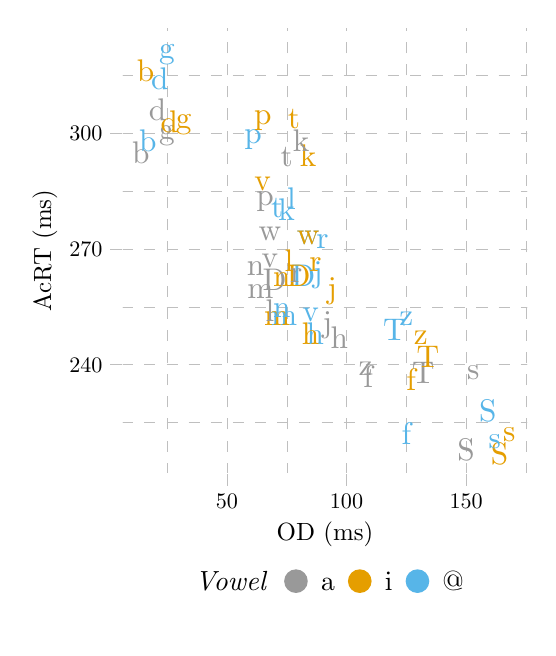
\begin{tikzpicture}[x=1pt,y=1pt]
\definecolor[named]{fillColor}{rgb}{1.00,1.00,1.00}
\path[use as bounding box,fill=fillColor,fill opacity=0.00] (0,0) rectangle (180.67,216.81);
\begin{scope}
\path[clip] (  0.00,  0.00) rectangle (180.67,216.81);
\definecolor[named]{fillColor}{rgb}{1.00,1.00,1.00}

\path[fill=fillColor] ( -0.00,  0.00) rectangle (180.67,216.81);
\end{scope}
\begin{scope}
\path[clip] ( 34.18, 55.61) rectangle (180.67,216.81);
\definecolor[named]{drawColor}{rgb}{1.00,1.00,1.00}

\path[draw=drawColor,line width= 0.6pt,line join=round,line cap=round] ( 34.18, 55.61) rectangle (180.68,216.81);
\definecolor[named]{drawColor}{rgb}{0.75,0.75,0.75}

\path[draw=drawColor,line width= 0.1pt,dash pattern=on 4pt off 4pt ,line join=round] ( 34.18, 74.10) --
	(180.67, 74.10);

\path[draw=drawColor,line width= 0.1pt,dash pattern=on 4pt off 4pt ,line join=round] ( 34.18,115.97) --
	(180.67,115.97);

\path[draw=drawColor,line width= 0.1pt,dash pattern=on 4pt off 4pt ,line join=round] ( 34.18,157.84) --
	(180.67,157.84);

\path[draw=drawColor,line width= 0.1pt,dash pattern=on 4pt off 4pt ,line join=round] ( 34.18,199.71) --
	(180.67,199.71);

\path[draw=drawColor,line width= 0.1pt,dash pattern=on 4pt off 4pt ,line join=round] ( 50.35, 55.61) --
	( 50.35,216.81);

\path[draw=drawColor,line width= 0.1pt,dash pattern=on 4pt off 4pt ,line join=round] ( 93.59, 55.61) --
	( 93.59,216.81);

\path[draw=drawColor,line width= 0.1pt,dash pattern=on 4pt off 4pt ,line join=round] (136.83, 55.61) --
	(136.83,216.81);

\path[draw=drawColor,line width= 0.1pt,dash pattern=on 4pt off 4pt ,line join=round] (180.07, 55.61) --
	(180.07,216.81);

\path[draw=drawColor,line width= 0.2pt,dash pattern=on 4pt off 4pt ,line join=round] ( 34.18, 95.04) --
	(180.67, 95.04);

\path[draw=drawColor,line width= 0.2pt,dash pattern=on 4pt off 4pt ,line join=round] ( 34.18,136.91) --
	(180.67,136.91);

\path[draw=drawColor,line width= 0.2pt,dash pattern=on 4pt off 4pt ,line join=round] ( 34.18,178.78) --
	(180.67,178.78);

\path[draw=drawColor,line width= 0.2pt,dash pattern=on 4pt off 4pt ,line join=round] ( 71.97, 55.61) --
	( 71.97,216.81);

\path[draw=drawColor,line width= 0.2pt,dash pattern=on 4pt off 4pt ,line join=round] (115.21, 55.61) --
	(115.21,216.81);

\path[draw=drawColor,line width= 0.2pt,dash pattern=on 4pt off 4pt ,line join=round] (158.45, 55.61) --
	(158.45,216.81);
\definecolor[named]{drawColor}{rgb}{0.90,0.62,0.00}

\node[text=drawColor,anchor=base,inner sep=0pt, outer sep=0pt, scale=  1.13] at (170.56, 59.03) {\textipa{S}};
\definecolor[named]{drawColor}{rgb}{0.60,0.60,0.60}

\node[text=drawColor,anchor=base,inner sep=0pt, outer sep=0pt, scale=  1.13] at (158.45, 60.43) {\textipa{S}};
\definecolor[named]{drawColor}{rgb}{0.34,0.71,0.91}

\node[text=drawColor,anchor=base,inner sep=0pt, outer sep=0pt, scale=  1.13] at (168.83, 64.62) {\textipa{s}};

\node[text=drawColor,anchor=base,inner sep=0pt, outer sep=0pt, scale=  1.13] at (136.83, 66.01) {\textipa{f}};
\definecolor[named]{drawColor}{rgb}{0.90,0.62,0.00}

\node[text=drawColor,anchor=base,inner sep=0pt, outer sep=0pt, scale=  1.13] at (174.02, 67.41) {\textipa{s}};
\definecolor[named]{drawColor}{rgb}{0.34,0.71,0.91}

\node[text=drawColor,anchor=base,inner sep=0pt, outer sep=0pt, scale=  1.13] at (166.23, 74.39) {\textipa{S}};
\definecolor[named]{drawColor}{rgb}{0.90,0.62,0.00}

\node[text=drawColor,anchor=base,inner sep=0pt, outer sep=0pt, scale=  1.13] at (138.56, 85.55) {\textipa{f}};
\definecolor[named]{drawColor}{rgb}{0.60,0.60,0.60}

\node[text=drawColor,anchor=base,inner sep=0pt, outer sep=0pt, scale=  1.13] at (122.99, 86.95) {\textipa{f}};

\node[text=drawColor,anchor=base,inner sep=0pt, outer sep=0pt, scale=  1.13] at (142.88, 88.34) {\textipa{T}};

\node[text=drawColor,anchor=base,inner sep=0pt, outer sep=0pt, scale=  1.13] at (161.04, 89.74) {\textipa{s}};

\node[text=drawColor,anchor=base,inner sep=0pt, outer sep=0pt, scale=  1.13] at (122.13, 91.13) {\textipa{z}};
\definecolor[named]{drawColor}{rgb}{0.90,0.62,0.00}

\node[text=drawColor,anchor=base,inner sep=0pt, outer sep=0pt, scale=  1.13] at (144.61, 93.93) {\textipa{T}};
\definecolor[named]{drawColor}{rgb}{0.60,0.60,0.60}

\node[text=drawColor,anchor=base,inner sep=0pt, outer sep=0pt, scale=  1.13] at (112.61,100.90) {\textipa{h}};
\definecolor[named]{drawColor}{rgb}{0.34,0.71,0.91}

\node[text=drawColor,anchor=base,inner sep=0pt, outer sep=0pt, scale=  1.13] at (103.97,102.30) {\textipa{h}};
\definecolor[named]{drawColor}{rgb}{0.90,0.62,0.00}

\node[text=drawColor,anchor=base,inner sep=0pt, outer sep=0pt, scale=  1.13] at (142.02,102.30) {\textipa{z}};

\node[text=drawColor,anchor=base,inner sep=0pt, outer sep=0pt, scale=  1.13] at (102.24,102.30) {\textipa{h}};
\definecolor[named]{drawColor}{rgb}{0.34,0.71,0.91}

\node[text=drawColor,anchor=base,inner sep=0pt, outer sep=0pt, scale=  1.13] at (132.51,103.69) {\textipa{T}};
\definecolor[named]{drawColor}{rgb}{0.60,0.60,0.60}

\node[text=drawColor,anchor=base,inner sep=0pt, outer sep=0pt, scale=  1.13] at (108.29,106.49) {\textipa{j}};
\definecolor[named]{drawColor}{rgb}{0.34,0.71,0.91}

\node[text=drawColor,anchor=base,inner sep=0pt, outer sep=0pt, scale=  1.13] at ( 92.72,109.28) {\textipa{m}};

\node[text=drawColor,anchor=base,inner sep=0pt, outer sep=0pt, scale=  1.13] at (136.83,109.28) {\textipa{z}};
\definecolor[named]{drawColor}{rgb}{0.90,0.62,0.00}

\node[text=drawColor,anchor=base,inner sep=0pt, outer sep=0pt, scale=  1.13] at ( 90.13,109.28) {\textipa{m}};
\definecolor[named]{drawColor}{rgb}{0.34,0.71,0.91}

\node[text=drawColor,anchor=base,inner sep=0pt, outer sep=0pt, scale=  1.13] at (102.24,110.67) {\textipa{v}};
\definecolor[named]{drawColor}{rgb}{0.60,0.60,0.60}

\node[text=drawColor,anchor=base,inner sep=0pt, outer sep=0pt, scale=  1.13] at ( 87.54,110.67) {\textipa{l}};
\definecolor[named]{drawColor}{rgb}{0.34,0.71,0.91}

\node[text=drawColor,anchor=base,inner sep=0pt, outer sep=0pt, scale=  1.13] at ( 91.86,112.07) {\textipa{n}};
\definecolor[named]{drawColor}{rgb}{0.60,0.60,0.60}

\node[text=drawColor,anchor=base,inner sep=0pt, outer sep=0pt, scale=  1.13] at ( 84.08,119.05) {\textipa{m}};
\definecolor[named]{drawColor}{rgb}{0.90,0.62,0.00}

\node[text=drawColor,anchor=base,inner sep=0pt, outer sep=0pt, scale=  1.13] at (110.02,119.05) {\textipa{j}};
\definecolor[named]{drawColor}{rgb}{0.60,0.60,0.60}

\node[text=drawColor,anchor=base,inner sep=0pt, outer sep=0pt, scale=  1.13] at ( 89.26,121.84) {\textipa{D}};
\definecolor[named]{drawColor}{rgb}{0.34,0.71,0.91}

\node[text=drawColor,anchor=base,inner sep=0pt, outer sep=0pt, scale=  1.13] at ( 99.64,123.23) {\textipa{D}};
\definecolor[named]{drawColor}{rgb}{0.90,0.62,0.00}

\node[text=drawColor,anchor=base,inner sep=0pt, outer sep=0pt, scale=  1.13] at ( 91.86,123.23) {\textipa{n}};

\node[text=drawColor,anchor=base,inner sep=0pt, outer sep=0pt, scale=  1.13] at ( 97.91,123.23) {\textipa{D}};
\definecolor[named]{drawColor}{rgb}{0.34,0.71,0.91}

\node[text=drawColor,anchor=base,inner sep=0pt, outer sep=0pt, scale=  1.13] at (104.83,124.63) {\textipa{j}};
\definecolor[named]{drawColor}{rgb}{0.60,0.60,0.60}

\node[text=drawColor,anchor=base,inner sep=0pt, outer sep=0pt, scale=  1.13] at ( 97.05,124.63) {\textipa{r}};

\node[text=drawColor,anchor=base,inner sep=0pt, outer sep=0pt, scale=  1.13] at ( 82.35,127.42) {\textipa{n}};
\definecolor[named]{drawColor}{rgb}{0.90,0.62,0.00}

\node[text=drawColor,anchor=base,inner sep=0pt, outer sep=0pt, scale=  1.13] at ( 94.45,128.82) {\textipa{l}};

\node[text=drawColor,anchor=base,inner sep=0pt, outer sep=0pt, scale=  1.13] at (103.97,128.82) {\textipa{r}};
\definecolor[named]{drawColor}{rgb}{0.60,0.60,0.60}

\node[text=drawColor,anchor=base,inner sep=0pt, outer sep=0pt, scale=  1.13] at ( 87.54,130.21) {\textipa{v}};
\definecolor[named]{drawColor}{rgb}{0.34,0.71,0.91}

\node[text=drawColor,anchor=base,inner sep=0pt, outer sep=0pt, scale=  1.13] at (106.56,137.19) {\textipa{r}};

\node[text=drawColor,anchor=base,inner sep=0pt, outer sep=0pt, scale=  1.13] at (101.37,138.59) {\textipa{w}};
\definecolor[named]{drawColor}{rgb}{0.90,0.62,0.00}

\node[text=drawColor,anchor=base,inner sep=0pt, outer sep=0pt, scale=  1.13] at (101.37,138.59) {\textipa{w}};
\definecolor[named]{drawColor}{rgb}{0.60,0.60,0.60}

\node[text=drawColor,anchor=base,inner sep=0pt, outer sep=0pt, scale=  1.13] at ( 87.54,139.98) {\textipa{w}};
\definecolor[named]{drawColor}{rgb}{0.34,0.71,0.91}

\node[text=drawColor,anchor=base,inner sep=0pt, outer sep=0pt, scale=  1.13] at ( 93.59,146.96) {\textipa{k}};

\node[text=drawColor,anchor=base,inner sep=0pt, outer sep=0pt, scale=  1.13] at ( 90.13,148.36) {\textipa{t}};

\node[text=drawColor,anchor=base,inner sep=0pt, outer sep=0pt, scale=  1.13] at ( 95.32,151.15) {\textipa{l}};
\definecolor[named]{drawColor}{rgb}{0.60,0.60,0.60}

\node[text=drawColor,anchor=base,inner sep=0pt, outer sep=0pt, scale=  1.13] at ( 85.81,152.54) {\textipa{p}};
\definecolor[named]{drawColor}{rgb}{0.90,0.62,0.00}

\node[text=drawColor,anchor=base,inner sep=0pt, outer sep=0pt, scale=  1.13] at ( 84.94,158.13) {\textipa{v}};
\definecolor[named]{drawColor}{rgb}{0.60,0.60,0.60}

\node[text=drawColor,anchor=base,inner sep=0pt, outer sep=0pt, scale=  1.13] at ( 93.59,166.50) {\textipa{t}};
\definecolor[named]{drawColor}{rgb}{0.90,0.62,0.00}

\node[text=drawColor,anchor=base,inner sep=0pt, outer sep=0pt, scale=  1.13] at (101.37,166.50) {\textipa{k}};
\definecolor[named]{drawColor}{rgb}{0.60,0.60,0.60}

\node[text=drawColor,anchor=base,inner sep=0pt, outer sep=0pt, scale=  1.13] at ( 40.84,167.90) {\textipa{b}};
\definecolor[named]{drawColor}{rgb}{0.34,0.71,0.91}

\node[text=drawColor,anchor=base,inner sep=0pt, outer sep=0pt, scale=  1.13] at ( 43.43,172.08) {\textipa{b}};
\definecolor[named]{drawColor}{rgb}{0.60,0.60,0.60}

\node[text=drawColor,anchor=base,inner sep=0pt, outer sep=0pt, scale=  1.13] at ( 98.78,172.08) {\textipa{k}};
\definecolor[named]{drawColor}{rgb}{0.34,0.71,0.91}

\node[text=drawColor,anchor=base,inner sep=0pt, outer sep=0pt, scale=  1.13] at ( 81.48,174.87) {\textipa{p}};
\definecolor[named]{drawColor}{rgb}{0.60,0.60,0.60}

\node[text=drawColor,anchor=base,inner sep=0pt, outer sep=0pt, scale=  1.13] at ( 50.35,176.27) {\textipa{g}};
\definecolor[named]{drawColor}{rgb}{0.90,0.62,0.00}

\node[text=drawColor,anchor=base,inner sep=0pt, outer sep=0pt, scale=  1.13] at ( 51.21,179.06) {\textipa{d}};

\node[text=drawColor,anchor=base,inner sep=0pt, outer sep=0pt, scale=  1.13] at ( 56.40,180.46) {\textipa{g}};

\node[text=drawColor,anchor=base,inner sep=0pt, outer sep=0pt, scale=  1.13] at ( 96.18,180.46) {\textipa{t}};

\node[text=drawColor,anchor=base,inner sep=0pt, outer sep=0pt, scale=  1.13] at ( 84.94,181.85) {\textipa{p}};
\definecolor[named]{drawColor}{rgb}{0.60,0.60,0.60}

\node[text=drawColor,anchor=base,inner sep=0pt, outer sep=0pt, scale=  1.13] at ( 46.89,183.25) {\textipa{d}};
\definecolor[named]{drawColor}{rgb}{0.34,0.71,0.91}

\node[text=drawColor,anchor=base,inner sep=0pt, outer sep=0pt, scale=  1.13] at ( 47.75,194.41) {\textipa{d}};
\definecolor[named]{drawColor}{rgb}{0.90,0.62,0.00}

\node[text=drawColor,anchor=base,inner sep=0pt, outer sep=0pt, scale=  1.13] at ( 42.57,197.20) {\textipa{b}};
\definecolor[named]{drawColor}{rgb}{0.34,0.71,0.91}

\node[text=drawColor,anchor=base,inner sep=0pt, outer sep=0pt, scale=  1.13] at ( 50.35,205.58) {\textipa{g}};
\definecolor[named]{drawColor}{rgb}{1.00,1.00,1.00}

\path[draw=drawColor,line width= 0.6pt,line join=round,line cap=round] ( 34.18, 55.61) rectangle (180.68,216.81);
\end{scope}
\begin{scope}
\path[clip] (  0.00,  0.00) rectangle (180.67,216.81);
\definecolor[named]{drawColor}{rgb}{0.00,0.00,0.00}

\node[text=drawColor,anchor=base east,inner sep=0pt, outer sep=0pt, scale=  0.80] at ( 27.06, 92.28) {240};

\node[text=drawColor,anchor=base east,inner sep=0pt, outer sep=0pt, scale=  0.80] at ( 27.06,134.15) {270};

\node[text=drawColor,anchor=base east,inner sep=0pt, outer sep=0pt, scale=  0.80] at ( 27.06,176.02) {300};
\end{scope}
\begin{scope}
\path[clip] (  0.00,  0.00) rectangle (180.67,216.81);
\definecolor[named]{drawColor}{rgb}{0.75,0.75,0.75}

\path[draw=drawColor,line width= 0.2pt,line join=round] ( 29.91, 95.04) --
	( 34.18, 95.04);

\path[draw=drawColor,line width= 0.2pt,line join=round] ( 29.91,136.91) --
	( 34.18,136.91);

\path[draw=drawColor,line width= 0.2pt,line join=round] ( 29.91,178.78) --
	( 34.18,178.78);
\end{scope}
\begin{scope}
\path[clip] (  0.00,  0.00) rectangle (180.67,216.81);
\definecolor[named]{drawColor}{rgb}{0.75,0.75,0.75}

\path[draw=drawColor,line width= 0.2pt,line join=round] ( 71.97, 51.34) --
	( 71.97, 55.61);

\path[draw=drawColor,line width= 0.2pt,line join=round] (115.21, 51.34) --
	(115.21, 55.61);

\path[draw=drawColor,line width= 0.2pt,line join=round] (158.45, 51.34) --
	(158.45, 55.61);
\end{scope}
\begin{scope}
\path[clip] (  0.00,  0.00) rectangle (180.67,216.81);
\definecolor[named]{drawColor}{rgb}{0.00,0.00,0.00}

\node[text=drawColor,anchor=base,inner sep=0pt, outer sep=0pt, scale=  0.80] at ( 71.97, 42.99) {50};

\node[text=drawColor,anchor=base,inner sep=0pt, outer sep=0pt, scale=  0.80] at (115.21, 42.99) {100};

\node[text=drawColor,anchor=base,inner sep=0pt, outer sep=0pt, scale=  0.80] at (158.45, 42.99) {150};
\end{scope}
\begin{scope}
\path[clip] (  0.00,  0.00) rectangle (180.67,216.81);
\definecolor[named]{drawColor}{rgb}{0.00,0.00,0.00}

\node[text=drawColor,anchor=base,inner sep=0pt, outer sep=0pt, scale=  0.90] at (107.43, 31.37) {OD (ms)};
\end{scope}
\begin{scope}
\path[clip] (  0.00,  0.00) rectangle (180.67,216.81);
\definecolor[named]{drawColor}{rgb}{0.00,0.00,0.00}

\node[text=drawColor,rotate= 90.00,anchor=base,inner sep=0pt, outer sep=0pt, scale=  0.90] at (  8.44,136.21) {AcRT (ms)};
\end{scope}
\begin{scope}
\path[clip] (  0.00,  0.00) rectangle (180.67,216.81);
\definecolor[named]{fillColor}{rgb}{1.00,1.00,1.00}

\path[fill=fillColor] ( 56.26,  5.31) rectangle (158.60, 28.30);
\end{scope}
\begin{scope}
\path[clip] (  0.00,  0.00) rectangle (180.67,216.81);
\definecolor[named]{drawColor}{rgb}{0.00,0.00,0.00}

\node[text=drawColor,anchor=base west,inner sep=0pt, outer sep=0pt, scale=  1.00] at ( 60.52, 13.36) {\itshape Vowel};
\end{scope}
\begin{scope}
\path[clip] (  0.00,  0.00) rectangle (180.67,216.81);

\path[] ( 89.71,  9.58) rectangle (104.16, 24.03);
\end{scope}
\begin{scope}
\path[clip] (  0.00,  0.00) rectangle (180.67,216.81);
\definecolor[named]{fillColor}{rgb}{0.60,0.60,0.60}

\path[fill=fillColor] ( 96.94, 16.81) circle (  4.27);
\end{scope}
\begin{scope}
\path[clip] (  0.00,  0.00) rectangle (180.67,216.81);

\path[] (112.78,  9.58) rectangle (127.23, 24.03);
\end{scope}
\begin{scope}
\path[clip] (  0.00,  0.00) rectangle (180.67,216.81);
\definecolor[named]{fillColor}{rgb}{0.90,0.62,0.00}

\path[fill=fillColor] (120.00, 16.81) circle (  4.27);
\end{scope}
\begin{scope}
\path[clip] (  0.00,  0.00) rectangle (180.67,216.81);

\path[] (133.62,  9.58) rectangle (148.08, 24.03);
\end{scope}
\begin{scope}
\path[clip] (  0.00,  0.00) rectangle (180.67,216.81);
\definecolor[named]{fillColor}{rgb}{0.34,0.71,0.91}

\path[fill=fillColor] (140.85, 16.81) circle (  4.27);
\end{scope}
\begin{scope}
\path[clip] (  0.00,  0.00) rectangle (180.67,216.81);
\definecolor[named]{drawColor}{rgb}{0.00,0.00,0.00}

\node[text=drawColor,anchor=base west,inner sep=0pt, outer sep=0pt, scale=  1.00] at (105.97, 13.36) {\textipa{a}};
\end{scope}
\begin{scope}
\path[clip] (  0.00,  0.00) rectangle (180.67,216.81);
\definecolor[named]{drawColor}{rgb}{0.00,0.00,0.00}

\node[text=drawColor,anchor=base west,inner sep=0pt, outer sep=0pt, scale=  1.00] at (129.04, 13.36) {\textipa{i}};
\end{scope}
\begin{scope}
\path[clip] (  0.00,  0.00) rectangle (180.67,216.81);
\definecolor[named]{drawColor}{rgb}{0.00,0.00,0.00}

\node[text=drawColor,anchor=base west,inner sep=0pt, outer sep=0pt, scale=  1.00] at (149.88, 13.36) {\textipa{@}};
\end{scope}
\end{tikzpicture}

    \end{column}
  \end{columns}
}


\frame{\frametitle{Revisiting the definitions and some differences}

Just so that we know what we mean by these acronyms. As far as I can tell this
is how the different intervals in different articles -- including
\cite{Jouen:MERP:2021} -- relate to each other:

\begin{center}
  \hspace*{-.5cm}
  \includegraphics[width=1.1\textwidth]{AAI_EAI_BAI.drawio.png}
\end{center}
}


\frame{\frametitle{Research question}

  The inverse correlation pattern was first reported by
  \cite{Fowler:PC:1979} with the regression coefficient also roughly
  -0.5. So, this begs the question:
  \vspace{.5cm}
  
  \centering
  {
    \large
    \usebeamercolor[fg]{title}
    Where does that inverse correlation
    pattern come from?
  }
}


\frame{
  \centering
  {
    \vfill

    \bf \Large 
    \usebeamercolor[fg]{title}
    Materials
    
    \vfill
  }
}

\frame{\frametitle{Experiment}
  \begin{itemize}
  \item Partially replicates, but also expands the materials of the
    experiment by \cite{Rastle:CME:2005}.
  \item Expands methods by adding ultrasound recording.
  \item /CCCVC/, /CCVC/, /CVC/, and /VC/ English lexical words were
    produced by two female speakers and one male speaker of Standard
    Scottish English.
  \item Measured with 2D ultrasound tongue imaging (at 120~fps) and
    synchronised sound recording.
  \end{itemize}
}

\frame{\frametitle{Problems}

  \begin{itemize}
  \item Segmentation is time and sanity consuming.
  \item Video segmentation might be faster than one would first think,
    but it is definetely at least as sanity consuming as one would
    think.
  \item Human annotators are inconsistent.
  \item Computer assisted segmentation can ease all of these problems.
  \end{itemize}
}

\frame{
  \centering
  {
    \vfill

    \bf \Large 
    \usebeamercolor[fg]{title}
    Method
    
    \vfill
  }
}

\frame{\frametitle{Background of the method}
  \begin{itemize}
  \item The analysis methods presented here are similar to methods
    developed by
    \begin{itemize}
    \item \cite{McMillan:CIP:2010, Drake:AEI:2013} who used Euclidean
      distance on ultrasound frames and
    \item \cite{Raeesy:PDA:2011} who used a similar method on MRI
      data.
    \end{itemize}
  \item However, we exploit knowledge of how ultrasound scanning works
    to produce more fine grained analysis.
 \end{itemize}
}

\frame{\frametitle{How is ultrasound data produced?}

  \begin{itemize}
  \item An ultrasound pulse is sent out from the probe in one
    direction at a time.
  \item Echoes from that direction are listened to for a certain time
    (which depends on the probe and scanner settings).
  \item This produces one scanline.
  \item By repeating the process over a number of directions and
    interpolating the gathered data the system produces human
    readable images.
  \item The data is usually presented to humans in interpolated form.
  \end{itemize}

}

\frame{\frametitle{Regular, interpolated ultrasound and anatomy}
  \begin{center}
    \includegraphics[width=\textwidth]{figures/P2_lemon_1st_frame_anatomy}
  \end{center}
}

\frame{\frametitle{What is raw ultrasound data / probe return data?}  
  
  \begin{center}
    \includegraphics[width=\textwidth]{P2_lemon_1st_frame_fan}
  \end{center}
}

\frame{\frametitle{Algorithms: Pixel Difference (PD)} 

  \begin{itemize}
  \item Interpret each raw frame as a huge N-dimensional vector ($n =
    63\times256$ in our case).
  \item Calculate the Euclidean distances between these vectors.
  \item Result gives a holistic measure of change between two frames.
  \item The next slide will show that the resulting curves are easy to
    annotate manually -- and illustrates a typical case where manual
    video annotation gives a later movement onset time.
  \item Automatic annotation required an extra step (we'll get back to
    that in a moment).
  \end{itemize}

}

\frame{\frametitle{Algorithms: Pixel Difference (PD)} 

  \includegraphics[width=\columnwidth]{PD_metric_d1.pdf}
  % generated with source/PD_by_scanline/thesis_PD_chapter_batch.m

  \vspace{-.3cm}
  \includegraphics[width=\columnwidth]{PD_wav.pdf}
  
}

\frame{\frametitle{Algorithms 2: Scanline Based Pixel Difference (SBPD)} 
  \begin{itemize}
  \item Take each of the scanlines (63 in our case) as a smaller
    M-dimensional vector ($m = 256$ in our case).
  \item Calculate the Euclidean distances between corresponding
    scanlines between frames.
  \item Result gives a measure of change between two frames with
    location (in sagittal plane, back to front) presented by the
    scanline number.
  \item By applying dynamic time warping with a test function to each
    scanline's PD curve we get a vector of 63 onset times for each
    recording. 
  \item Taking the median of the individual onset candidates has
    proven to be a reliable way of automating onset detection
    \citep{Palo:MPS:2019}.
  \end{itemize}
}


\frame{
  \centering
  {
    \vfill

    \bf \Large 
    \usebeamercolor[fg]{title}
    Results
    
    \vfill
  }
}

\frame{\frametitle{Results: Acoustics}
  \begin{center}
    \vspace*{-.5cm}
    \hspace*{-1cm}
    \includegraphics[width=\textwidth]{figures/OD_vs_AcRT.jpg}
  \end{center}
  Medianised within participant, over several repetitions and over
  the vowels \textipa{/a,i,O/}. Over all analysable n = 1386: 439 from P1, 672 from P3, and
  275 from P4.  }

\frame{\frametitle{Results: AAI}
  \begin{center}
    \vspace*{-.5cm}
    \hspace*{-1cm}
    \includegraphics[width=\textwidth]{figures/OD_vs_AAI.jpg}
  \end{center}
  Medianised within participant, over several repetitions and over
  the vowels \textipa{/a,i,O/}. Over all analysable n = 1386: 439 from P1, 672 from P3,
  and 275 from P4.
}

\frame{\frametitle{Results: Statistical modelling}

  Fitting linear mixed models to the data with a step-up model
  selection procedure, we have for Acoustic Reaction
  Time\footnote{P-value $\approx 0.04548$ when comparing against a
    model without a trial term. Previous step -- adding RhymeDur --
    had a P-value $\approx 7.616\times 10^{-9}$.}:
  \begin{equation}
    AcRT \sim OD + RhymeDur + trial + (1|id) + (1|word), \label{acRTmod3}
  \end{equation}
  or as a (general) prediction model:
  \begin{equation}
    AcRT =  -0.42 \times OD + 0.20 \times RhymeDur + 0.06 \times trial. \label{acRTpred}
  \end{equation}

  And for Articulatory to Acoustic Interval (AAI)\footnote{P-value
    $\approx 0.0003768$ compared against a model without a trial
    term.}:
  \begin{equation}
    AAI \sim OD + RhymeDur + trial + (1|id) + (1|word), \label{AAImod3}
  \end{equation}
  or as a (general) prediction model:
  \begin{equation}
    AAI =  -0.40 \times OD + 0.31 \times RhymeDur + 0.12 \times trial. \label{AAIpred}
  \end{equation}
}

\frame{\frametitle{Results: Statistical modelling (continued)}

  \begin{itemize}
  \item Acoustic data repeats the general inverse correlation pattern
    of previous studies with some refinements.
  \item AAI repeats the correlation pattern and is likely its actual locus.
  \item No vowel quality effects were found.
  \item In contrast, articulatory reaction time could not be predicted with
    utterance duration variables and in particular did not have any
    statistically significant correlation with OD. Instead it seems to be a
    noisy constant $\approx$ 120~ms in this dataset.
  \end{itemize}
}



\frame{
  \centering
  {
    \vfill

    \bf \Large 
    \usebeamercolor[fg]{title}
    Tentative theory
    
    \vfill
  }
}

\frame{\frametitle{Effect of OD on AAI}
  \begin{center}
    \vspace*{-.5cm}
    \hspace*{-.5cm}
    \includegraphics[width=1.1\textwidth]{effect_of_OD.drawio.png}
  \end{center}
}

\frame{\frametitle{Effect of articulatory rate on AAI}
  \begin{center}
    \vspace*{-.5cm}
    \hspace*{-.5cm}
    \includegraphics[width=\textwidth]{effect_of_RhymeDur.drawio.png}
  \end{center}
}

\frame{\frametitle{Conclusions}

  \begin{itemize}
  \item The present results are in agreement with the literature in
    terms of acoustics.
  \item The inverse correlation pattern of Acoustic Reaction Time and Onset
  Duration originates int the inverse correlation of AAI and Onset Duration.
  \item The modelling results on AAI lead to the conclusion that, in
    terms of timing, the silent articulation preceding an utterance
    should be considered part of speech.
  \end{itemize}
}

\frame[allowframebreaks]{\frametitle{References}
  \scriptsize
  \bibliographystyle{apalike}
  \bibliography{bib/master,bib/jpalo}
}


\frame{
  \centering
  {
    \vfill

    \bf \Large 
    \usebeamercolor[fg]{title}
    Thank you!

  }
  \vspace{.3cm}

  Also many thanks to everybody who's helped along the way: Alan
  Wrench and Steve Cowen with data and recordings,\\
  my PhD supervisors Sonja Schaeffler and Jim Scobbie,\\
  my wonderful participants, and many many more.
    
  \vfill
}

\frame{\frametitle{Connection with speech cycling}
  \begin{center}
    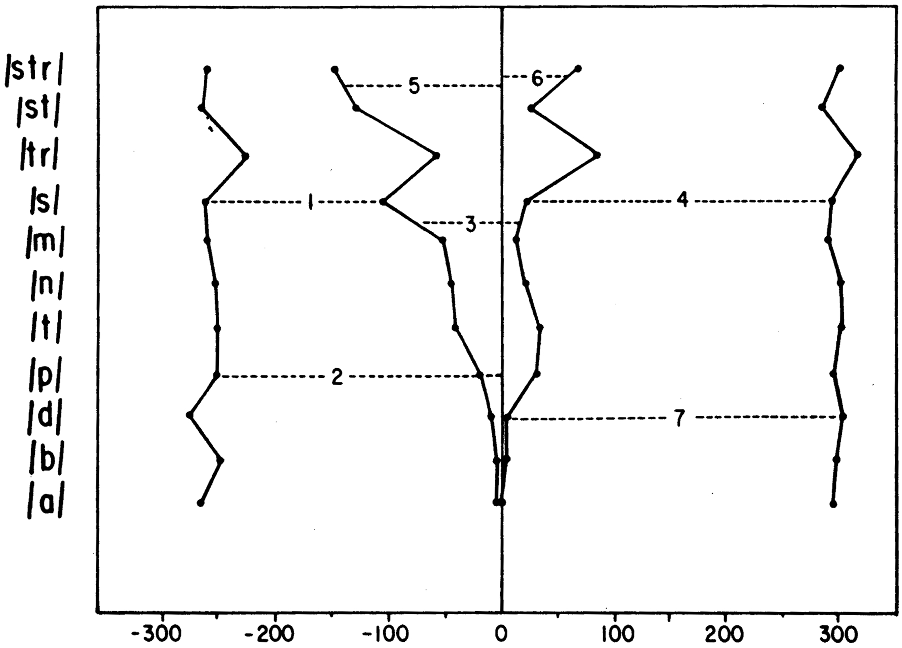
\includegraphics[width=.7\textwidth]{Fowler_cycling}
  \end{center}
  \begin{itemize}
  \item Figure from \cite{Fowler:NMC:1981}.
  \item Metronome click at 0 ms.
  \item Relevant intervals are: 1. silence between words, 3. onset
    consonant, and 4. vowel.
  \end{itemize}
}

\frame{\frametitle{Annotating Pixel Difference (PD)} 

  \begin{center}
    \hspace*{-1.3cm}
    \includegraphics[width=1.18\textwidth]{pd_annotation.png}
  \end{center}

}

\frame{\frametitle{SBPD and anatomy}

  The SBPD-gram on the rigth shows change over time for each
  scanline.
  \vspace{.5cm}

  \begin{center}
    \includegraphics[width=\textwidth]{figures/anatomy_to_SBPD}
  \end{center}
}

\frame{\frametitle{Examples of PD and SBPD}

  \hspace*{-.12\textwidth}\includegraphics[width = 1.2\textwidth]{ultrafest1.eps}

  \hspace*{-.12\textwidth}\includegraphics[width = 1.2\textwidth]{ultrafest2.eps}
}

\frame{\frametitle{Analysing location of first movement}
  \begin{itemize}
  \item Calculate SBPD for each token.
  \item Run DTW for each scanline of each token.
  \item Merge data from acoustic annotation, manual annotation and
    SBPD/DTW analysis.
  \item Remove tokens that were manually identified as false starts.
  \item Take median of onsets identified by DTW over tokens for each scanline.
  \item Plot results.
  \item (Scratch head.)
  \end{itemize}
}

\frame{%\frametitle{Results: Participant 1}
  \begin{center}
    \vspace*{-.5cm}
    \hspace*{-1cm}
    \includegraphics[width=1.18\textwidth]{P1_zoomed.pdf}
  \end{center}
}

\frame{%\frametitle{Results: Participant 3}
  \begin{center}
    \vspace*{-.5cm}
    \hspace*{-1cm}
    \includegraphics[width=1.18\textwidth]{P3_zoomed.pdf}
  \end{center}
}

\frame{%\frametitle{Results: Participant 4}
  \begin{center}
    \vspace*{-.5cm}
    \hspace*{-1cm}
    \includegraphics[width=1.18\textwidth]{P4_zoomed.pdf}
  \end{center}
}

\frame{%\frametitle{Results: Participant 1}
  \begin{center}
    \vspace*{-.5cm}
    \hspace*{-1cm}
    \includegraphics[width=1.18\textwidth]{P1_cloud.pdf}
  \end{center}
}

\frame{%\frametitle{Results: Participant 3}
  \begin{center}
    \vspace*{-.5cm}
    \hspace*{-1cm}
    \includegraphics[width=1.18\textwidth]{P3_cloud.pdf}
  \end{center}
}

\frame{%\frametitle{Results: Participant 4}
  \begin{center}
    \vspace*{-.5cm}
    \hspace*{-1cm}
    \includegraphics[width=1.18\textwidth]{P4_cloud.pdf}
  \end{center}
}


\frame{\frametitle{Relation of an interpolated ultrasound frame to anatomy}
  \begin{center}
    \includegraphics[width=.45\textwidth]{figures/DA_and_P1_overlay_2.jpg}
    \includegraphics[width=.45\textwidth]{figures/DA_and_P1_overlay_3.jpg}
  \end{center}
}


\end{document}

